% Thanks to Kevin D. McGrath for the presentation template.
\documentclass{beamer}

% Packages.
\usepackage{amsmath}
\usepackage{color}
\usepackage{graphicx}
\usepackage{tikz}

\usetikzlibrary[arrows.meta,backgrounds,fit]

% Hyperlinks.
\def\name{Wade Cline}
\hypersetup{
  colorlinks = true,
  citecolor = black,
  linkcolor = black,
  urlcolor = black,
  pdfauthor = {\name},
  pdftitle = {Introduction to IRC},
  pdfsubject = {Introduction to IRC},
  pdfpagemode = UseNone
}

% ???
\usetheme[hideothersubsections]{Hannover}
\usecolortheme{sidebartab}

% Presentation metadata.
\title[IRC Intro]{Introduction to IRC via \texttt{irssi}}
\author{Wade Cline}

%\AtBeginSection[]
%{
%  \begin{frame}<beamer>{Outline}
%    \tableofcontents[currentsection]
%  \end{frame}
%}
%\AtBeginSubsection[]
%{
%  \begin{frame}<beamer>{Outline}
%    % \transwipe
%    \tableofcontents[currentsection,currentsubsection]
%  \end{frame}
%}

\begin{document}

% Title.
\begin{frame}
  \titlepage
\end{frame}

% Table of Contents.
\begin{frame}{Outline}
	% TODO: Words here.
	% \transwipe
	\tableofcontents
	% You might wish to add the option [pausesections]
	Examples in \texttt{irssi}
\end{frame}

\section{About}

\begin{frame}{IRC}
\begin{itemize}
	% IRC stands for "Internet Relay Chat".
	\item Internet Relay Chat (IRC)
	% IRC is a protocol for real-time textual communication between groups of users.
	\item Real-time, text-based chat for groups
	% Some advantages of IRC are:
	\begin{itemize}
		% The specifications are open.  This means that anyone may write either a server or a client program implementing the specifications.
		\item Open specifications
		\begin{itemize}
			\item RFC 1459 (Internet Relay Chat Protocol)
			\item RFC 2810 (Internet Relay Chat: Architecture)
			\item RFC 2811 (Internet Relay Chat: Channel Management)
			\item RFC 2812 (Internet Relay Chat: Client Protocol)
			\item RFC 2813 (Internet Relay Chat: Server Protocol)
		\end{itemize}
		% There are many Free Software implementations of both clients and servers.  This means that one can run their own server without interference by an outside party requiring their own Terms of Service or licensing scheme.
		\item Free Software implementations
		\begin{itemize}
			\item Clients: \textbf{\texttt{irssi}}, \texttt{weechat}, HexChat, KiwiIRC, \&c.
			\item Servers: InspIRCd, \texttt{ircd-seven}, UnrealIRCd, Charybdis, \&c.
		\end{itemize}
		% Due to its longevity, the protocol is stable, so one can write programs, such as bots, and expect them to work consistently.
		\item Stable protocol
		% The protocol is minimalistic.  This is because the Internet was much more bandwidth and latency constrained when the protocol was written.  Nowadays this means that we can easily run IRC clients and/or servers on small devices, such as SBCs (Single Board Computers) like the Beagle Bone or Raspberry Pi, or minimal servers such as the $5/month options provided by Linode and Digital Ocean.
		\item Minimal
	\end{itemize}
\end{itemize}
\end{frame}

\section{Topology}

\begin{frame}{Topology}
\begin{itemize}
	% IRC services are divided into networks.  Example networks include: Freenode, OFTC, CAT.
	\item Each IRC service is a separate \emph{network} (Ex: Freenode, OFTC, PDXCAT)
	% Each network has one or more servers associated with it.
	\item A network consists of one or more \emph{servers} (Ex: \texttt{orwell.freenode.net}, \texttt{card.freenode.net}, \texttt{barjavel.freenode.net})
	% Servers within a network are joined together in a topology known as a "Spanning Tree".  Below is a hypothetical example of the Freenode network.  The letters represent the order in which the servers were joined to the network.  Note how each server joins the one nearest to it rather than joining the last one attached to the network.
	\item Servers arranged in a \emph{spanning tree} topology.  Hypothetical Freenode network with servers joined in order \texttt{A} - \texttt{F}: \\
	\begin{center}
	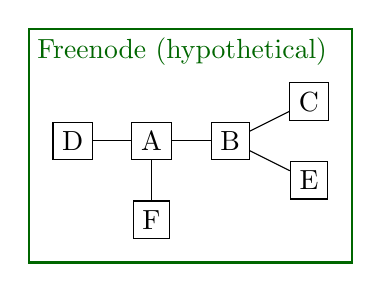
\begin{tikzpicture}
		\node(A) [draw] at (0, 0) {A};
		\node(B) [draw] at (1, 0) {B};
		\node(C) [draw] at (2, 0.5) {C};
		\node(D) [draw] at (-1, 0) {D};
		\node(E) [draw] at (2, -0.5) {E};
		\node(F) [draw] at (0, -1) {F};
		\node(padding) at (0,1) {};
		\draw (A) -- (B);
		\draw (B) -- (C);
		\draw (A) -- (D);
		\draw (B) -- (E);
		\draw (A) -- (F);
		\begin{scope}[on background layer]
			\node (bback) [rectangle,thick,draw=green!40!black,inner sep=0.3cm,fit=(A) (B) (C) (D) (E) (F) (padding)] {};
			\node [below right,text=green!40!black] at (bback.north west) {Freenode (hypothetical)};
		\end{scope}
	\end{tikzpicture}
	\end{center}
\end{itemize}
\end{frame}

\begin{frame}{Connecting}
\begin{itemize}
	% In order to connect to the network, a client needs only connect to a single server which belongs to the network.  The server then acts as the gateway to the entire network for the client.
	\item \emph{Clients} (such as \texttt{irssi}) connect to individual servers, and thus join the network.
	% We'll demonstrate by connecting to the Freenode network.  Begin by running the 'irssi' program.
	\item Begin by running \texttt{irssi}.
	% First, we configure the Freenode network.
	\item Configure the Freenode network: \texttt{/network add freenode}.
	% Then we add the server via which we wish to access the Freenode network.  Though the Freenode network consists of many servers to chose from, the easiest way is to use 'chat.freenode.net', which selects a server for you.
	\item Add a server to the network:  \texttt{/server add -network freenode chat.freenode.net}
	% Finally, we connect to the network.
	\item Connect to the network: \texttt{/connect freenode}
	% If all goes well then we will have connected to the Freenode network and be presented with the server's MotD.
	\item Server will display its Message of the Day (MotD)
	% Having to manually connect to the server isn't very convenient, so we can configure 'irssi' to automatically connect to it on startup.
	\item Auto-connect on startup via \texttt{/server add -auto chat.freenode.net}
	% We can confirm that this works by closing the program and then re-launching it as so.
	\item Close with \texttt{/exit}, then rerun via \texttt{irssi}.
\end{itemize}
\end{frame}

\section{Interface}

\begin{frame}{\texttt{irssi} interface}
	% This is an example of the 'irssi' interface after successfully logging into the Freenode network.  What each of these areas means is covered in the next slide.
	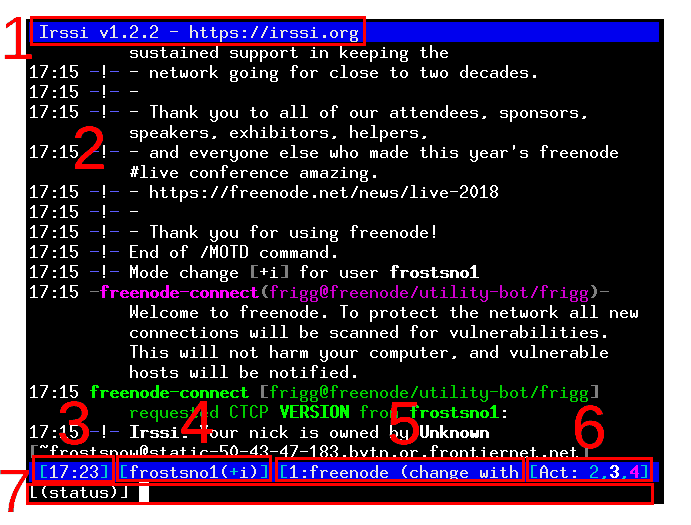
\includegraphics[scale=1.75]{win1.png}
\end{frame}

\begin{frame}{\texttt{irssi} interface (cont.)}
\begin{enumerate}
	% The bar at the top displays the current version of your 'irssi' client.
	\item Client version
	% This large panel in the middle displays the text relevant to that particular window.  In this example we can see the end of the MotD, followed by some messages from Freenode regarding their anti-spam measures, and an indication that the nickname I've selected is already is use.
	\item Window text
	% This leftmost section of the bottom bar shows the current local time.  This screenshot was taken at 5:23 p.m. local time.
	\item Current time
	% This displays the user's nickname and their current user modes.  This currently shows my nickname as "frostsno1" and my mode as "+i".  We'll be discussing nicknames shortly and modes later.
	\item Nickname and user modes
	% This displays the current window number on the left, currently "1", followed by the current network selection, currently "freenode".
	\item Window number and current network.
	% The rightmost section of the bottom bar displays which windows currently have unread activity.  The number indicates which window has activity and the color indicates what kind of activity the windows has.  Light blue denotes only informational messages such as users joining and parting, white means that users have been sending chat messages, and purple means that someone has mentioned you explicitly.
	\item Window numbers containing \textbf{act}ivity.
	\begin{itemize}
		\item Light blue: Informational messages
		\item White: Chat messages
		\item Purple: Messaging \emph{you}
	\end{itemize}
	% The final item on the bottom is where you compose both messages and commands.
	\item Input bar
\end{enumerate}
\end{frame}

\begin{frame}{Users}
\begin{itemize}
	% The person who is running the client is known as the *user*, after all, they are *using* the client.
	\item Person running client known as the \emph{user}.
	% The user is identified by a network-unique *nickname*, or *nick*, which is sometimes referred to as a *handle*.  This is the most important identifier for a user, though a couple extra pieces of information are also sent.
	\item \emph{User} identified in IRC by \emph{nickname}, or "nick"
	\begin{itemize}
		\item Also known as \emph{handle}
		\item The most important identifier
		\item Set via \texttt{/nick <name>}
	\end{itemize}
	% The 'ident' is the name of the user's account on their local machine.  Since these days people are the administrators of their own machines, this identifier is far less important than it once was and can almost always be spoofed by the user's client software.
	\item Additional \emph{ident} entry is username on user's machine.
	% The same goes for the 'realname' parameter, though some users, especially on Freenode, configure this as their actual real name when contributing to projects.
	\item Last, \emph{realname} is user's actual name.
\end{itemize}
\end{frame}

\begin{frame}[fragile=singleslide]{User info}
\begin{itemize}
	% You can use the '/whois' command in order to view information about users.  This can also be used to view information about yourself.
	\item \texttt{/whois <nick>} (and \texttt{/whowas}) to view user information
	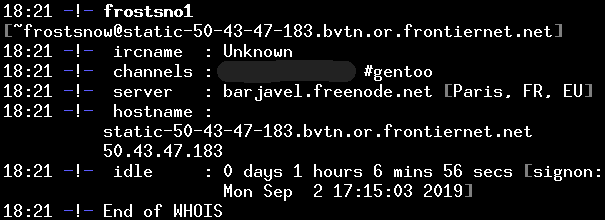
\includegraphics[scale=1.75]{whois.png}
	% At the top of the output is the nickname and hostmask of the user.  The hostmask is used to help identify users beyond just their nickname.  Most networks do some kind of obfuscation on this by default, but Freenode does not.
	\item Topmost: Nickname \verb|[|ident@hostmask\verb|]|
	\begin{itemize}
		\item Hostmask identifies users, often obfuscated by default (but not on Freenode)
	\end{itemize}
	% The 'ircname' can be used to display your realname in case you are interested in providing it.
	\item \texttt{ircname}: User's real name (\texttt{settings} - \texttt{core} - \texttt{real\_name} in \texttt{.irssi/config})
	% This next section lists which channels a user is joined to; we will be covering channels shortly.  Note that the full list may or may not be displayed depending the user's modes.
	\item Channels user is joined to (not always displayed)
	% Other information such as the user's account, their client certificate fingerprint, TLS usage, &c. may also be displayed here.
	\item Other information (accounts, cert fingerprint, \&c.)
\end{itemize}
\end{frame}

\section{Chatting}

\begin{frame}{Channels}
\begin{itemize}
	% The primary means of communication in IRC is the *channel*.  Users join channels and then use them in order to talk to members of the channel.
	\item Groups of users communicate over \emph{channels}
	% Each channel name is prefixed by a '#'.  In Freenode, which is a topical network for Free/Open Source Software, "off-topic" channels are prefixed by a '##' as a matter of custom.
	\item Channel \emph{names} are prefixed by a \#
	\begin{itemize}
		\item \#\# prefix for "off-topic" channels in Freenode
	\end{itemize}
	% You enter channels by *joining* them, done by the '/join' command with the channel name as its argument.
	\item Enter a channel by \emph{joining} it (\texttt{/join <name>})
	\begin{itemize}
		\item Ex: \texttt{/join \#osu-lug}
	\end{itemize}
	% Almost every channel has a *topic* which will provide useful metadata about the channel.  You can view it manually by running '/topic'.
	\item Channel \emph{topic} provides information (\texttt{/topic})
	% You can also view the list of users currently joined to the channel by running the '/names' command.
	\item View user list with \texttt{/names}
	% When are you done in a channel you can leave it by *parting* it, done with the '/part' command.
	\item Leave a channel by \emph{parting} it (\texttt{/part})
\end{itemize}
\end{frame}

\begin{frame}
	% This is an example of what 'irssi' looks like after joining a channel, in this case the '#osu-lug' channel on Freenode.  Note that several locations now display different information than they did previously.
	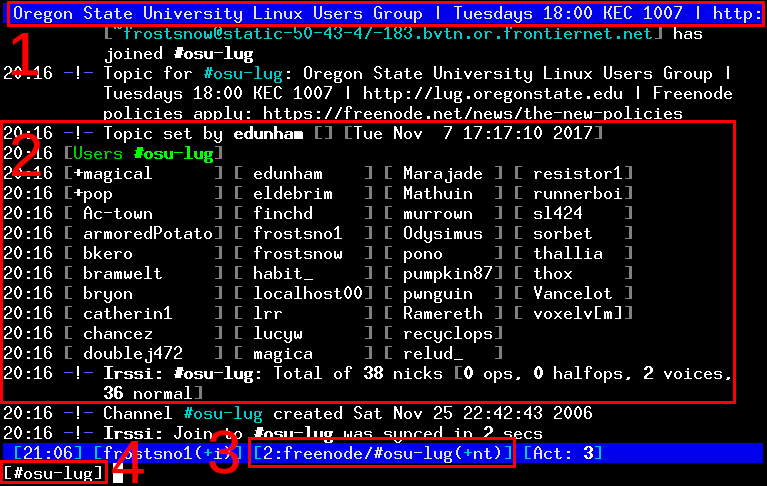
\includegraphics[scale=1.5]{join.png}
	\begin{enumerate}
		% The channel topic is now displayed in the top bar rather than the client version.  Some topics are too long to display properly up here, so remember that you can use '/topic' in order to print it to the main area.
		\item Channel topic (\texttt{/topic} to view long topics)
		% The user list is displayed when you join; should you need to see it again, run '/names'.
		\item Channel users (\texttt{/names} if you forget)
		% Note how the channel number has changed from '1' to '2'.  In addition, the channel name is now displayed after the network name with channel modes, covered later, following it.
		\item Window number:network/channel name(channel modes)
		% The prompt at the bottom left now informs you which channel you will be chatting in.
		\item Channel
	\end{enumerate}
\end{frame}

\begin{frame}{Examples}
	% Up top is an example of chatting in 'irssi'.  Each line corresponds to a bullet point below.
	\begin{center}
	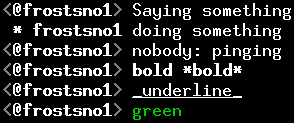
\includegraphics[scale=1.75]{chatting.png}
	\end{center}
	\begin{enumerate}
		% First, one can simply type stuff in order to chat.
		\item Type words for raw text
		% One can also perform an "action" by prefixing their text with the '/me' command.  Games such as World of Warcraft have an equivalent "emote" (/e) command.
		\item \texttt{/me} command for actions (emotes)
		% If one wants to draw the attention of a specific user they can "ping" said user by beginning their sentence with the user's name, followed immediately by a colon, and then the text to send that user.
		\item \emph{pinging} a user (tab-complete their name)
		% The following modifications do not work on all channels.
		% You can use Ctrl+B to delimit sections which should user boldface font.  You can also surround a *single* word with asterisks in order to emphasize that word and it will automatically be made bold.
		\item Bold with Ctrl+B or asterisks
		% Likewise, you can also underline a *single* word by surrounding it with underscores.
		\item Underline with underscores
		% You can also send text in color, though you generally shouldn't, by using Ctrl+C followed by the number of the mIRC color code which you wish to use.  Color codes can usually be found in the below directory or thereabouts.
		\item Ctrl+C+\# for mIRC color codes
		\begin{itemize}
			\item Codes: \texttt{/usr/share/doc/irssi/formats.txt}
		\end{itemize}
	\end{enumerate}
\end{frame}

\begin{frame}{Misc.}
\begin{itemize}
	% You may have noticed that upon joining a channel 'irssi' automatically switched windows for you.  You can change windows manually by running '/window #', or, depending on your terminal, press Alt+#.
	\item Change windows with \texttt{/window \#} (or Alt+\#)
	% In addition, you probably don't want to manually join all channels that you're interested in each time you open 'irssi', so you can have it automatically join a channel at start-up with the below command.
	\item Auto-join channel: \texttt{/channel add -auto <channel> <network>}
	\begin{itemize}
		\item Ex: \texttt{/channel add -auto \#osu-lug freenode}
	\end{itemize}
	% Should you need to find channels, you can list channels on the network with '/list', but be warned that large networks such as Freenode will flood you with information and disconnect you.
	\item List network channels with \texttt{/list}
	\begin{itemize}
		\item Warning: Don't use on Freenode due to channel count
	\end{itemize}
	% Not all conversation is done through channels.  You can directly message users with the '/msg' command, but note that it's generally rude to directly message users unless they ask you to.
	\item Direct message a nick via \texttt{/msg <nick>}
	\begin{itemize}
		\item Also known as a \emph{Private Message} (PM)
		\item Generally considered rude unless invited
	\end{itemize}
	% Unlike many modern protocols, IRC, without extensions, does not save chat history.  You can, however, have your client save any history that you experience locally by using the below command.
	\item History not saved by default
	\begin{itemize}
		\item Save locally with: \texttt{/set autolog on}
	\end{itemize}
\end{itemize}
\end{frame}

\section{Modes}

\begin{frame}{About}
\begin{itemize}
	% Modes are basically configuration settings that change how the IRC protocol behaves.
	\item Modes are like configuration settings
	% Each mode is represented by a single, case-sensitive letter.
	\item Represented by a single, case-sensitive letter
	% There are two kinds of modes: "user modes", which are applied to a given user, and "channel modes" which are applied to a given channel.
	\item Two kinds: \emph{user modes} and \emph{channel modes}
	% Some modes accept a parameter; this is most common (only?) with channel modes, which modifies how the channel behaves for a particular user or a particular group of users.
	\item Certain modes are \emph{parameterized}
	% Modes tend to vary between networks.  Although a few modes are standardized, many are not.
	\item Mode list may vary between networks
	% You will thus probably want to look up the modes, but, be careful: the '/help mode' command list help text that is built into the 'irssi' software, but the software can't know about every non-standard mode in existence!  A better option is often to ask the server directly by running the below commands for user modes and channel modes, respectively.  Note that not all servers can be queried with a 'help' command.
	\item \texttt{/help mode} vs \texttt{/quote help umode} and \texttt{/quote help cmode}
	% Many modes are settable via *services*, which we will discuss later.
	\item Many are configurable via \emph{services}
\end{itemize}
\end{frame}

\begin{frame}{User mode examples}
\begin{itemize}
	% Here are some examples of modes that you might see.
	% The "invisible" mode means that users who do not share a common channel with the user will not be able to see the user in '/who' output.  Note that, with regards to the '/whois' command, this means that users will only see the user as joined to channels in which both users joined; the other channels will not be listed.
	\item \texttt{i}: invisible
	\begin{itemize}
		\item User not listed in \texttt{/who} unless "known"
	\end{itemize}
	% This mode makes it so that only users who have been registered with NickServ (discussed later) will be able to directly message the user.  This is mostly an anti-spam prevention measure.
	\item \texttt{R}: Registered DMs only (Freenode-specific)
	\begin{itemize}
		\item Only registered users may direct-message the user
	\end{itemize}
	% This means that the user has established a secure connection to the server.  SSL/TLS connections will be discussed briefly later.
	\item \texttt{Z}: Secure connection (Freenode-specific)
	\begin{itemize}
		\item User connected via SSL/TLS
	\end{itemize}
	% This means that the user is an IRC operator.  IRC operators often have the power to ban users from the entire network and the responsibility to enforce the rules of the network.  Treat them with the proper respect :).
	\item \texttt{o}: IRC Operator (IRCop)
	\begin{itemize}
		\item User is an IRC operator
	\end{itemize}
\end{itemize}
\end{frame}

\begin{frame}{Channel mode examples}
\begin{itemize}
	% Channel mode '+t' prevents regular users from setting the topic.  This tends to be enabled on all but the most casual channels.
	\item \texttt{t}: Topic lock
	\begin{itemize}
		\item Only channel operators may set channel topic
	\end{itemize}
	% Channel mode '+s' makes the channel a "secret" channel, in that it is not listed by the usual commands.  Note that this is simplistic obscurity and doesn't offer any real security.  This is usually used by casual, off-topic channels.
	\item \texttt{s}: Secret channel
	\begin{itemize}
		\item Channel not shown in \texttt{/list}, \texttt{/whois}, \&c.
	\end{itemize}
	% Channel mode '+c' strips color codes from channel messages.  Many users consider colored output to be annoying, and it's a favorite of spammers, hence many channels have color disabled.
	\item \texttt{c}: Strip color
	\begin{itemize}
		\item Remove color codes from channel messages
	\end{itemize}
	% Channel mode '+i' means that users may only join the channel if they've been invited.  This is actually secure in contrast to '+s'.
	\item \texttt{i}: Invite-only
	\begin{itemize}
		\item Users must be explicitly invited to the channel (\texttt{/invite})
	\end{itemize}
	% Channel mode '+m' means that the channel is "moderated" in that only *voiced* users (discussed later) will be able to speak in the channel.  This is useful if you want a channel where many people can speak but only a select group can listen.
	\item \texttt{m}: Moderated channel
	\begin{itemize}
		\item Only users with \texttt{+v} may speak in channel.
	\end{itemize}
\end{itemize}
\end{frame}

\begin{frame}{More channel mode examples}
\begin{itemize}
	% Note that the below channel modes all have parameters attached to them.
	% First and most important is the '+o' channel mode, which grants the specified users "operator" privileges on the channel; this means that the user can do things such as kick, ban, and otherwise modify the channel.  These users are usually recognizable by the '@' which is prefixed to their user name, but note that the Freenode network discourages channel operators from idling in this mode, and hence channel operators often won't leave this mode "on" unless they need to perform an action that requires the aforementioned mode.
	\item \texttt{o <nick>}: Channel operator
	\begin{itemize}
		\item User is a \emph{channel operator} (ChanOP; kicking, banning, \&c.)
		\item Name usually prefixed by the \emph{hat} `\texttt{@}'
		\item Often ``off'' on Freenode channels
	\end{itemize}
	% The '+v' channel mode allows certain users to talk on a moderated channel.  These users tend to be noticeable for the '+' hat next to their nickname.
	\item \texttt{v <nick>}: Voiced user
	\begin{itemize}
		\item User can speak in moderated channel
		\item Hat: \texttt{+}
	\end{itemize}
	% The '+b' channel mode is used to prevent users from joining a channel.  Note the format of the parameter is much more complex than a simple nickname; this allows banning of entire IP ranges instead of playing whack-a-mole with users doing nickname hopping.  A full discuss of this format is outside the scope of this discussion.
	\item \texttt{b <nick!ident@host>} Banned user
	\begin{itemize}
		\item User cannot join the channel
	\end{itemize}
\end{itemize}
\end{frame}

\section{Services}

\begin{frame}{Rationale}
\begin{itemize}
	% Here is where things get tricky and IRC's age begins to show.  Modern services usually have an initial registration step where you reserve a name and authenticate yourself with a password before being able to interact with them.  IRC, on the other hand, simply checks a nickname for uniqueness *when it connects* and has no authenticate step, meaning someone could easily use "your" nickname as you have no claim to it unless you are actively connected.
	\item IRC's default "registration"
	\begin{itemize}
		\item Only checks for immediate usage collision
		\item No authentication
		\item Easily claimed by another
	\end{itemize}
	% Similar issues arise with channel ownership.  For example, when all channel operators disconnect from a channel, no one can can be promoted to channel operator status; the channel becomes forever unmoderated until all users disconnect and then someone re-creates it.  In addition, all channel statuses such as its topic are destroyed when all users leave a channel.
	\item IRC's default channel ownership
	\begin{itemize}
		\item What happens when all ChanOps disconnect?
		\item What happens when all users disconnect?
	\end{itemize}
	% In order to fix these problems, a feature called *services* were created.
	\item \emph{Services} fix these problems
\end{itemize}
\end{frame}

\begin{frame}{About}
\begin{itemize}
	% A *service* is essentially a program-controlled user, or *bot*, that has special privileges.
	\item \emph{Service} a program-controlled user, or \emph{bot}, with special privileges
	% Most, if not all, services provide different nicknames for different purposes.  A couple of examples services, which we will be covering, are listed below.  Many service packages provide additional services as well.
	\item Different nicknames for different purposes, examples:
	\begin{itemize}
		\item \texttt{NickServ}: Account (nickname) management
		\item \texttt{ChanServ}: Channel management
		\item \texttt{MemoServ}: Offline user messaging
	\end{itemize}
	% You can interact with services as you do regular users, by messaging them!  Of course, since these are programs, you send them specially-formatted messages which they interpret as commands rather than chatting with them about what you had for lunch today.  Sending a service the 'help' message will give you a list of available commands that the service supports.
	\item Interact with them by direct messages
	\begin{itemize}
		\item Example: \texttt{/msg NickServ help} for usage
	\end{itemize}
	% A complication with services is that, like modes, different networks provide different services.  Almost all networks are similar with regards to 'NickServ' and 'ChanServ' basic functionality, but the additional features can vary quite a bit.
	\item Like modes, different networks provide different services
\end{itemize}
\end{frame}

\begin{frame}{\texttt{NickServ}}
\begin{itemize}
	% Nickserv is primarily used in order to create *accounts* which you can then associate and reserve nicknames with.
	\item Create \emph{accounts}, reserve nicknames
	% In order to create an account, you must choose the nickname you wish to have and then *register* it by providing 'NickServ' with a plaintext password and e-mail.  Most services will require you to confirm registration via a verification e-mail before registration will be complete.
	\item Register account: \texttt{register <password> <e-mail>}
	% Once your account has been registered, you then *identify* yourself by supplying the password for your nickname's account to 'NickServ'.  This is annoying to do manually, so you'll probably want to configure 'irssi' to do it for you with the below command.
	\item After connecting to the network, \emph{identify} yourself with \texttt{NickServ}
	\begin{itemize}
		\item Identify account: \texttt{identify <password>}
		\item Auto-identify in \texttt{irssi}: \texttt{/NETWORK ADD -autosendcmd "/msg nickserv identify <pass>; wait 2000" freenode}
	\end{itemize}
	% Now, should someone try to use your registered nickname, or should you have a stale session still active, you can kick the other session off with the 'ghost' command.
	\item Disconnect impersonators: \texttt{ghost <nick>}
	% Again, doing manual enforcement is tiresome, so you can also have 'NickServ' do it automatically with the below command.  Though I've yet to have anyone actually impersonate me, it does help me make sure that I'm properly configured to auto-identify when it kicks me off my nickname.
	\item Auto-disconnect impersonators: \texttt{set enforce on}
	% After 'NickServ' has renamed someone using your registered nickname while unauthorized, a temporary "enforcement" is placed on it which prevents all use of it.  When this is a result of your misconfiguration and the issue has been resolved, you may wish to remove the enforcement right away by using the 'release' command so that you can resume using your nickname.
	\item Remove enforcement hold: \texttt{release <nick>}
	% It's also worth knowing that you can view your account information via the 'info' command; you can also view the public information of other user's accounts this way.
	\item Show account info: \texttt{info <nick>}
	% You may also wish to toggle whether or not your e-mail is publicly viewable (I believe that it isn't by default).  This can be done with the 'set hidemail' command.
	\item Hide e-mail: \texttt{set hidemail on}
	% Lastly, rather than sending a password to 'NickServ' at connect time, you can supply a public certificate as part of an SSL/TLS connection; this certificate will be hashed into a *fingerprint* by services and can then be used in order to identify your account.  The 'cert add' command will add the fingerprint of the certificate that you are currently using to those which can identify your account.  We'll discuss SSL/TLS connections briefly later on.
	\item Identify via certificate \emph{fingerprint} (discussed later): \texttt{cert add}
\end{itemize}
\end{frame}

\begin{frame}{\texttt{ChanServ}}
\begin{itemize}
	% As 'NickServ' helps to manage nicknames via accounts, 'ChanServ' helps to manage channels by *registering* them to an account (thus you must be identified to services).  You can register a channel with the below command.  After creating a channel, it's important to register is right away, otherwise all operators might be disconnected and you'll be left unable to either register or manage the channel.
	\item Manage channels by \emph{registering} them
	\begin{itemize}
		\item Must be identified to services (i.e. \texttt{NickServ})
		\item \texttt{register <\#channel>}
		\item Register immediately after creation to prevent unmoderated channels
	\end{itemize}
	% An important aspect of registering a channel with 'ChanServ' is that the service will remember who has operating privileges, allowing you to enable and disable operator mode as you see fit.  Freenode encourages users to only use operator mode when it's necessary in order to maintain order in a channel.
	\item Registered channels retain operator status
	\begin{itemize}
		\item Set ChanOP mode: \texttt{OP <\#channel>}
		\item Unset ChanOP mode: \texttt{DEOP <\#channel>}
	\end{itemize}
	% You can also set the topic of a channel via a 'ChanServ' command rather than running the '/topic' command within a channel.
	\item Set channel topic: \texttt{topic <\#channel> <topic>}
	% If you are curious about the registration status of a particular channel, 'ChanServ' provides the '/info' command as well.
	\item Get information about a channel with \texttt{/info <\#channel>}
\end{itemize}
\end{frame}

\begin{frame}{\texttt{MemoServ}}
\begin{itemize}
	% Due IRC's mostly stateless nature, the protocol doesn't natively support messaging offline users.
	\item IRC doesn't allow messaging offline users
	% In order to work around this, the 'MemoServ' service allows messaging users who have registered accounts.
	\item \texttt{MemoServ} can store \& forward offline messages
	% While useful, this feature is actually relatively unknown, and the "unread memos" message isn't displayed particularly prominently, at least not the way 'irssi' displays it.
	\item Cons: relatively unknown, some people don't notice memos immediately
	% Nonetheless, they can still prove useful.  You can use the below command in order to send a memo...
	\item \texttt{send <nick> <message>} to send a memo
	% ...and you can read all of your new memos with the 'read new' command.
	\item \texttt{read new} to read new memos
\end{itemize}
\end{frame}

\section{Netsplits}

\begin{frame}{Overview}
\begin{itemize}
	% Due to IRC's low-latency, statelessness, and topology, it can suffer from something known as a *netsplit*, where one part of the network becomes disconnected from the other part.  This can happen as a result of poor network conditions, but it can also happen because of misconfigured servers in the network.
	\item Servers in the network can become disconnected, resulting in a \emph{netsplit}
\begin{figure}
	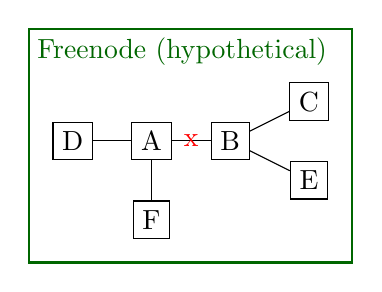
\begin{tikzpicture}
		\node(A) [draw] at (0, 0) {A};
		\node(B) [draw] at (1, 0) {B};
		\node(C) [draw] at (2, 0.5) {C};
		\node(D) [draw] at (-1, 0) {D};
		\node(E) [draw] at (2, -0.5) {E};
		\node(F) [draw] at (0, -1) {F};
		\node(padding) at (0,1) {};
		\draw (A) -- (B)
		node[pos=0.5,red](fail){x};
		\draw (B) -- (C);
		\draw (A) -- (D);
		\draw (B) -- (E);
		\draw (A) -- (F);
		\begin{scope}[on background layer]
			\node (bback) [rectangle,thick,draw=green!40!black,inner sep=0.3cm,fit=(A) (B) (C) (D) (E) (F) (padding)] {};
			\node [below right,text=green!40!black] at (bback.north west) {Freenode (hypothetical)};
		\end{scope}
	\end{tikzpicture}
\end{figure}
	% In the example above, the servers on the left have become disconnect from the servers on the right.
	\item Example: servers \texttt{A}, \texttt{D}, and \texttt{F} separated from \texttt{B}, \texttt{C}, and \texttt{E}
	% This means that a user on the 'A' server can only talk with users on the 'A', 'D', and 'F' servers, and the situation is analogous for a user connect to the 'B' server.
	\item Users can only chat with their side of the netsplit
	% This is a (poor) example of what a netsplit looks like in 'irssi'.  In this case the unfortunate 'finchd' was connected a server(s) that got disconnect from the network.  From their perspective, everyone else got netsplit.
	\item Example in \texttt{irssi}: 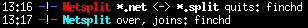
\includegraphics[scale=2.5]{netsplit_example.png}
	% There isn't much you can do about netsplit besides wait them out, or connect to a server that is on your desired side of the netsplit if you are able.
	\item Wait out netsplits, or connect to different server
\end{itemize}
\end{frame}

\section{SSL/TLS}

\begin{frame}{Overview}
\begin{itemize}
	% Now, a very brief overview of encrypted connections to IRC.  Connections are by default *unencrypted*, meaning that their contents can be viewed by anyone able to capture the network traffic.
	\item Connections are \emph{unencrypted} by default
	% The SSL/TLS protocol can be used to *encrypt* the client's IRC connection in order to prevent this.
	\item SSL/TLS connections are \emph{encrypted} (the 'S' in HTTPS)
	% TLS services are offered by most IRC networks on TCP port 6697 instead of the unencrypted 6667.
	\item TLS often offered on TCP port 66\textbf{9}7
	% The following options can be applied to the '/server' or '/connect' commands in order to use encrypted connections.  Note that I've divided the options up into two conceptual sections: the first sections is with regards to verifying the *server*, so that you know you are talking to the correct IRC server and not an imposter; the second is with regards to verifying *yourself* to the server, so that the server can easily identify you.
	\item Supply options to \texttt{/server} or \texttt{/connect}
	% With regards to verifying the server, the most important option is '-tls_verify', which ensures that the server presents a valid certificate.  Believe it or not, the inferior '-tls' option just accepts whatever certificate is passed to it, even if it's a bogus one.  Now, some servers use a self-signed certificate or one that is not part of your system's default *PKI* (Public Key Infrastructure) configuration; in this case you can tell 'irssi' to trust the certificate by pointing the '-tls_cafile' option to a copy of the server's certificate.
	\item Server verification options:
	\begin{itemize}
		\item \texttt{-tls\_verify}: Verify server's certificate
		\item \texttt{-tls\_cafile}: Use specific Certificate Authority (CA); useful for self-signed certs
	\end{itemize}
	% You can also pass your own certificate to the server.  This can be used in order to identify oneself to services as mentioned earlier.  The '-tls_cert' option specifies a path to the certificate file to be passed and the '-tls_pkey' option specifies the path for the certificates corresponding private key.  You can find more information on the OSU-LUG blog (http://lug.oregonstate.edu/blog/irc-and-ssl/).
	\item Client verification options:
	\begin{itemize}
		\item \texttt{-tls\_cert}: Client's certificate
		\item \texttt{-tks\_pkey}: Client's private key
	\end{itemize}
\end{itemize}
\end{frame}

\section{Questions}

\begin{frame}{The End!}
\begin{itemize}
	% Any questions?  You will be expected to know everything when the test comes.
	\item Any questions?
\end{itemize}
\end{frame}

\end{document}
